\documentclass[12pt]{article}

%----------------------------------------------------------------------------------------
%	SETTINGS
%----------------------------------------------------------------------------------------
\usepackage{amsmath}

\usepackage{float}
\usepackage{graphicx}
\usepackage[normal]{caption}
\usepackage{subcaption}
\usepackage{mathtools}

\setlength\parindent{24pt}

% Make numbering in the enumerate environment by letter rather than number (e.g. section 6)
\renewcommand{\labelenumi}{\alph{enumi}.}

%----------------------------------------------------------------------------------------
%	DOCUMENT INFORMATION
%----------------------------------------------------------------------------------------

\title{Robotics Project \\ Kalman Filter} % Title

\author{Hoang V. \textsc{Nguyen}, Lukas \textsc{Leung}, Zhuoming \textsc{Tan}} % Author name

\date{\today} % Date for the report

\begin{document}

	\maketitle % Insert the title, author and date

	\begin{center}
		\begin{tabular}{l r}
			Instructor: & Professor Ken Basye \\ % Instructor/supervisor
		\end{tabular}
	\end{center}

	% If you wish to include an abstract, uncomment the lines below
	% \begin{abstract}
	% Kalman filter.
	% \end{abstract}

	%----------------------------------------------------------------------------------------
	%	TABLE OF CONTENTS
	%----------------------------------------------------------------------------------------

	%\newpage
	%\tableofcontents
	%\newpage

	%----------------------------------------------------------------------------------------
	%	SECTION 1
	%----------------------------------------------------------------------------------------

	\section{Introduction}\label{sec:intro}

	In this project we will use Kalman filter to estimate the motion path of an aircraft. We are writing our program in python.

	\subsection{Physics model}\label{sub:model}
	The following model defines the state estimation:
	\begin{equation}
		\hat{\mathbf{x}}_t=\mathbf{A}\hat{\mathbf{x}}_{t-1}+\mathbf{B}\mathbf{u}_t+\mathbf{w}_{t-1}
	\end{equation}
	Which is
	\begin{equation}
		\begin{bmatrix}
			p^{(t)}_x \\ p^{(t)}_y \\ v^{(t)}_x \\ v^{(t)}_y
		\end{bmatrix}=
		\underbrace{\begin{bmatrix}
			1 & 0 & t & 0 \\
			0 & 1 & 0 & t \\
			0 & 0 & 1 & 0 \\
			0 & 0 & 0 & 1
		\end{bmatrix}}_{\text{state transition}}
		\begin{bmatrix}
			p^{(t-1)}_x \\ p^{(t-1)}_y \\ v^{(t-1)}_x \\ v^{(t-1)}_y
		\end{bmatrix}+
		\underbrace{\begin{bmatrix}
			t^2/2 & 0 \\
			0 & t^2/2 \\
			t & 0 \\
			0 & t
		\end{bmatrix}}_{\text{control matrix}}
		\begin{bmatrix}
			a^{(t-1)}_x \\ a^{(t-1)}_y
		\end{bmatrix}+\text{noise}
	\end{equation}
	whose $\text{noise}\sim\mathcal{N}\left(0,\Sigma_x\right)$. The state transition matrix $A$ and control matrix $B$ are what we use in the program. They are only dependent on $t$, here representing the time step, so are constant matricies if we run the program with a fixed time interval setting. And the following defines the observation from the state
	\begin{equation}
		\mathbf{z}_k=\mathbf{H}\hat{\mathbf{x}}_k+\text{noise}
	\end{equation}
	which is
	\begin{equation}
		\begin{bmatrix}
			p^{(t)}_x \\ p^{(t)}_y
		\end{bmatrix}=
		\underbrace{\begin{bmatrix}
			1 & 0 & 0 & 0 \\
			0 & 1 & 0 & 0
		\end{bmatrix}}_{\text{estimation model}}
		\begin{bmatrix}
			p_x \\ p_y \\ v_x \\ v_y
		\end{bmatrix}+\text{noise}
	\end{equation}
	whose $\text{noise}\sim\mathcal{N}\left(0,\Sigma_z\right)$. Because our estimation includes both position and velocity, but out measurement only has position, we have an measurement matrix $C$ to translate our measurement to estimation.

	\subsection{Prediction}\label{sub:predict}
	\begin{equation}
		p_t=\mathbf{A}p_{t-1}\mathbf{A}^T+Q
	\end{equation}
	where $Q$ is the convarience matrix of $E_x$.

	\subsection{Measure}\label{sub:measure}
	The Kalman gain would be
	\begin{equation}
		k_k=p_k\mathbf{H}^T{\left(\mathbf{H}p_k\mathbf{H}^T+R\right)}^{-1}
	\end{equation}
	where $R$ is the convarience matrix of $E_z$. The system noise covariance matrix:
	\begin{equation}
		Q=
		\begin{bmatrix}
			\sigma_1^2       &                  & \sigma_1\sigma_3 &                 \\
			                 & \sigma_2^2       &                  & \sigma_2\sigma4 \\
			\sigma_3\sigma_1 &                  & \sigma_3^2       &                 \\
			                 & \sigma_4\sigma_2 &                  & \sigma_4^2      \\
		\end{bmatrix}
	\end{equation}
	has been erased off the zero elements because we have assumed $x$ and $y$ velocities are independent.
	%----------------------------------------------------------------------------------------
	%	SECTION 2
	%----------------------------------------------------------------------------------------
	\section{Program}\label{sec:program}

	\subsection{Initial Conditions}\label{sub:Initial Conditions}
	The arguments we put into the program are explained below, with their sample default initial input.
	\begin{equation}
		\mathtt{true\_initial\_state}=
		\begin{bmatrix}
			p_{x0} \\ p_{y0} \\ v_{x0} \\ v_{y0}
		\end{bmatrix}=
		\begin{bmatrix}
			10 \\ 10 \\ 0 \\ 0
		\end{bmatrix}
	\end{equation}

	\begin{equation}
		\mathtt{initial\_estimation}=
		\begin{bmatrix}
			p_{x0} \\ p_{y0} \\ v_{x0} \\ v_{y0}
		\end{bmatrix}=
		\begin{bmatrix}
			0 \\ 0 \\ 0 \\ 0
		\end{bmatrix}
	\end{equation}

	\begin{equation}
			\mathtt{acceleration\_function\_x}=1
	\end{equation}

	\begin{equation}
			\mathtt{acceleration\_function\_y}=1
	\end{equation}

	\begin{equation}
			(\mathtt{int})\ \mathtt{number\_of\_iters}=10
	\end{equation}

	\begin{equation}
			(\mathtt{double})\ \mathtt{delta\_t}=1.0
	\end{equation}

	\begin{equation}
			\mathtt{sig\_acceleration}=
			\begin{bmatrix}
				\mathrm{std\_dev}(a_x) & \mathrm{std\_dev}(a_y)
			\end{bmatrix}=
			\begin{bmatrix}
				0.1 & 0.1
			\end{bmatrix}
	\end{equation}

	\begin{equation}
			\mathtt{var\_obs}=
			\begin{bmatrix}
				\mathrm{var}(\mathrm{observed}\_P_x) & 0 \\
				0 & \mathrm{var}(\mathrm{observed}\_P_y) \\
			\end{bmatrix}=
			\begin{bmatrix}
				1 & 0 \\
				0 & 1
			\end{bmatrix}
	\end{equation}

	\subsection{Process}\label{sub:Process}
	The program generates the noisy observations by adding random Gaussian noise to the true trajectory. Then through the run Kalman filter learns the error and tries to trace the real trajectory. Because it cannot measure the velocity of the object, the Kalman filter is working based on the measurement of the position of the object.

	\subsection{Example Run}\label{sub:Example Run}
	We put in the true initial state to be
	\[
		\mathtt{true\_initial\_state}=
		\begin{bmatrix}
			10 \\ 10 \\ 2 \\ 2
		\end{bmatrix}
	\]
	and the initial estimations are
	\[
		\mathtt{true\_initial\_state}=
		\begin{bmatrix}
			0 \\ 0 \\ 0 \\ 0
		\end{bmatrix}
	\]
	and the acceleration functions are now given as
	\[
		\mathtt{acceleration\_function\_x}=100\times\sin(x)
	\]
	\[
		\mathtt{acceleration\_function\_y}=-100\times\cos(x)
	\]
	The iterations
	\[
		\mathtt{number\_of\_iters}=50
	\]
	and standard deviation of accelerations
	\[
		\mathtt{sig\_acceleration}=
		\begin{bmatrix}
			2.5 & 2.5
		\end{bmatrix}
	\]

	%----------------------------------------------------------------------------------------
	%	SECTION 3
	%----------------------------------------------------------------------------------------
	\section{Conclusion}
	We have plotted within the program with \texttt{matplotlib}, and one of the runs and the graphs are included below. We have plotted the trajectory in the $xy$-plane, along with the estimation; and the difference between teh real and estimated values of the state vector.
	\begin{figure}[H]
		\centering
		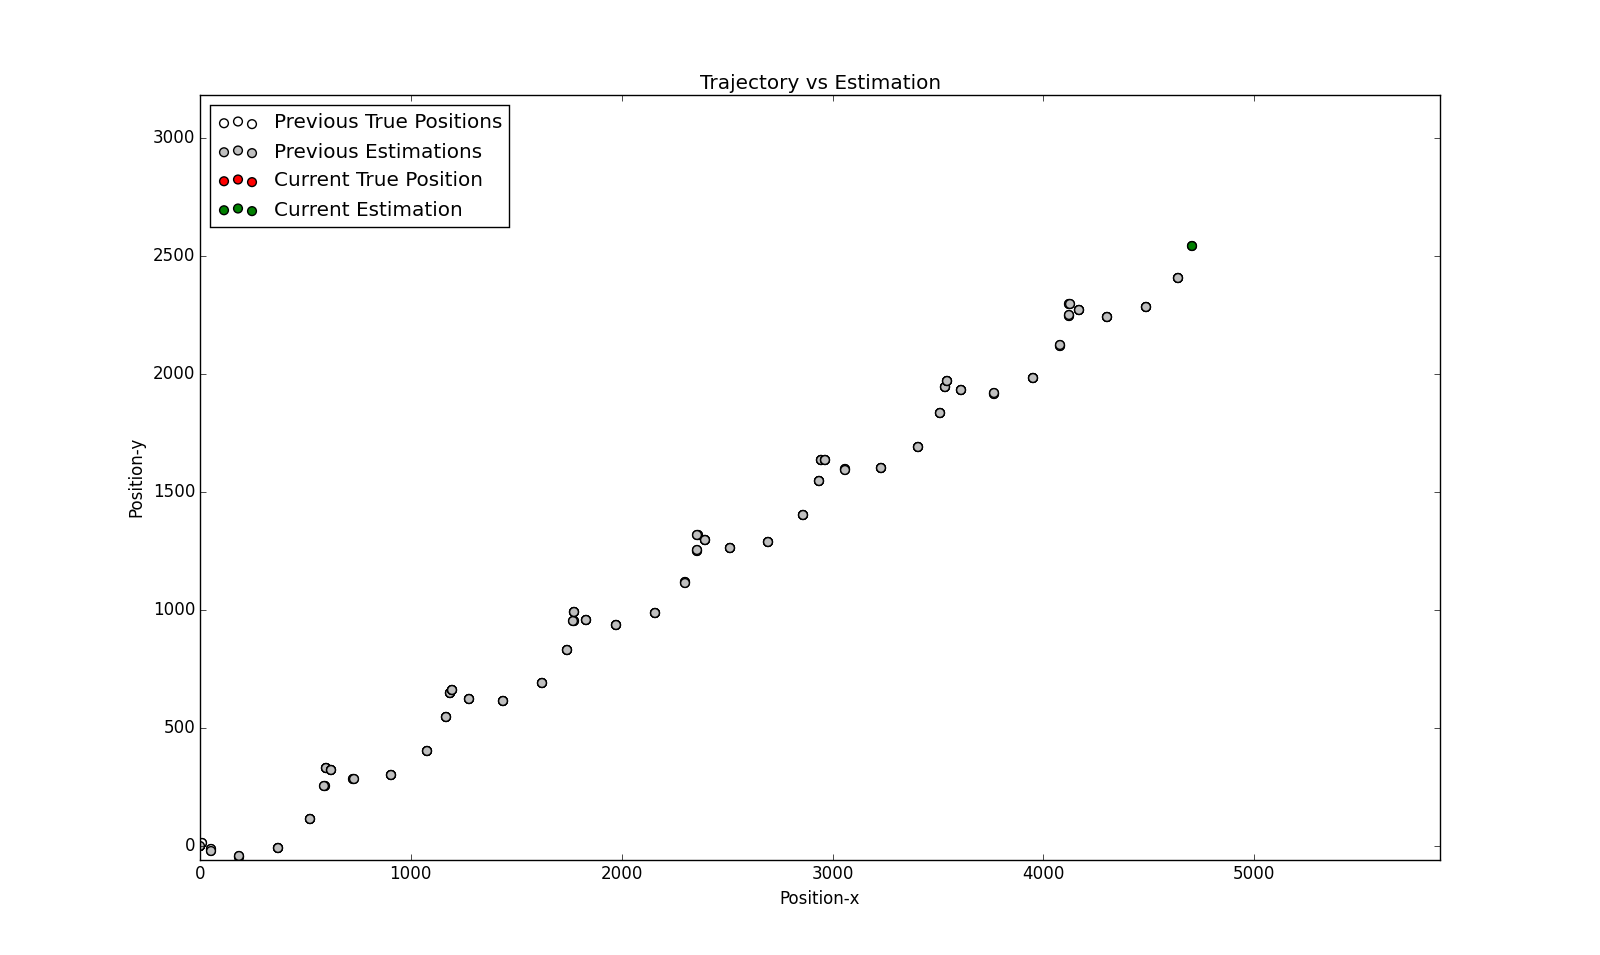
\includegraphics[width=\textwidth]{TvE}
		\caption{Trajectory versus Estimation}
	\end{figure}

	\begin{figure}[H]
		\centering
		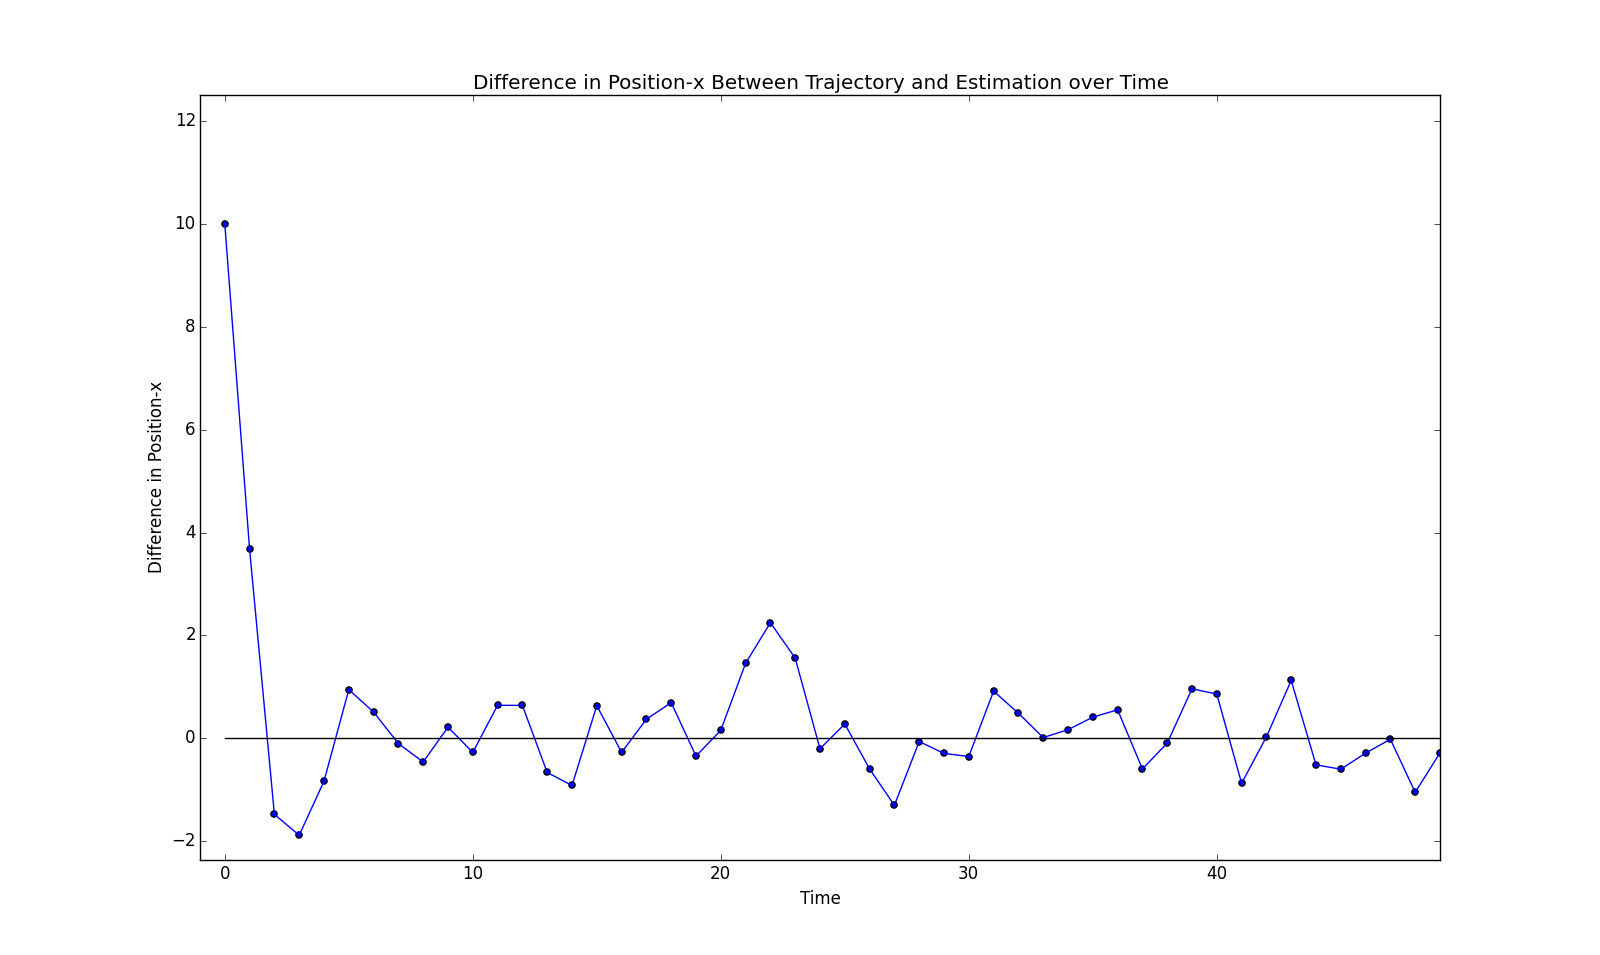
\includegraphics[width=\textwidth]{Diffpx}
		\caption{Difference between real and estimated $x$ position}
	\end{figure}

	\begin{figure}[H]
		\centering
		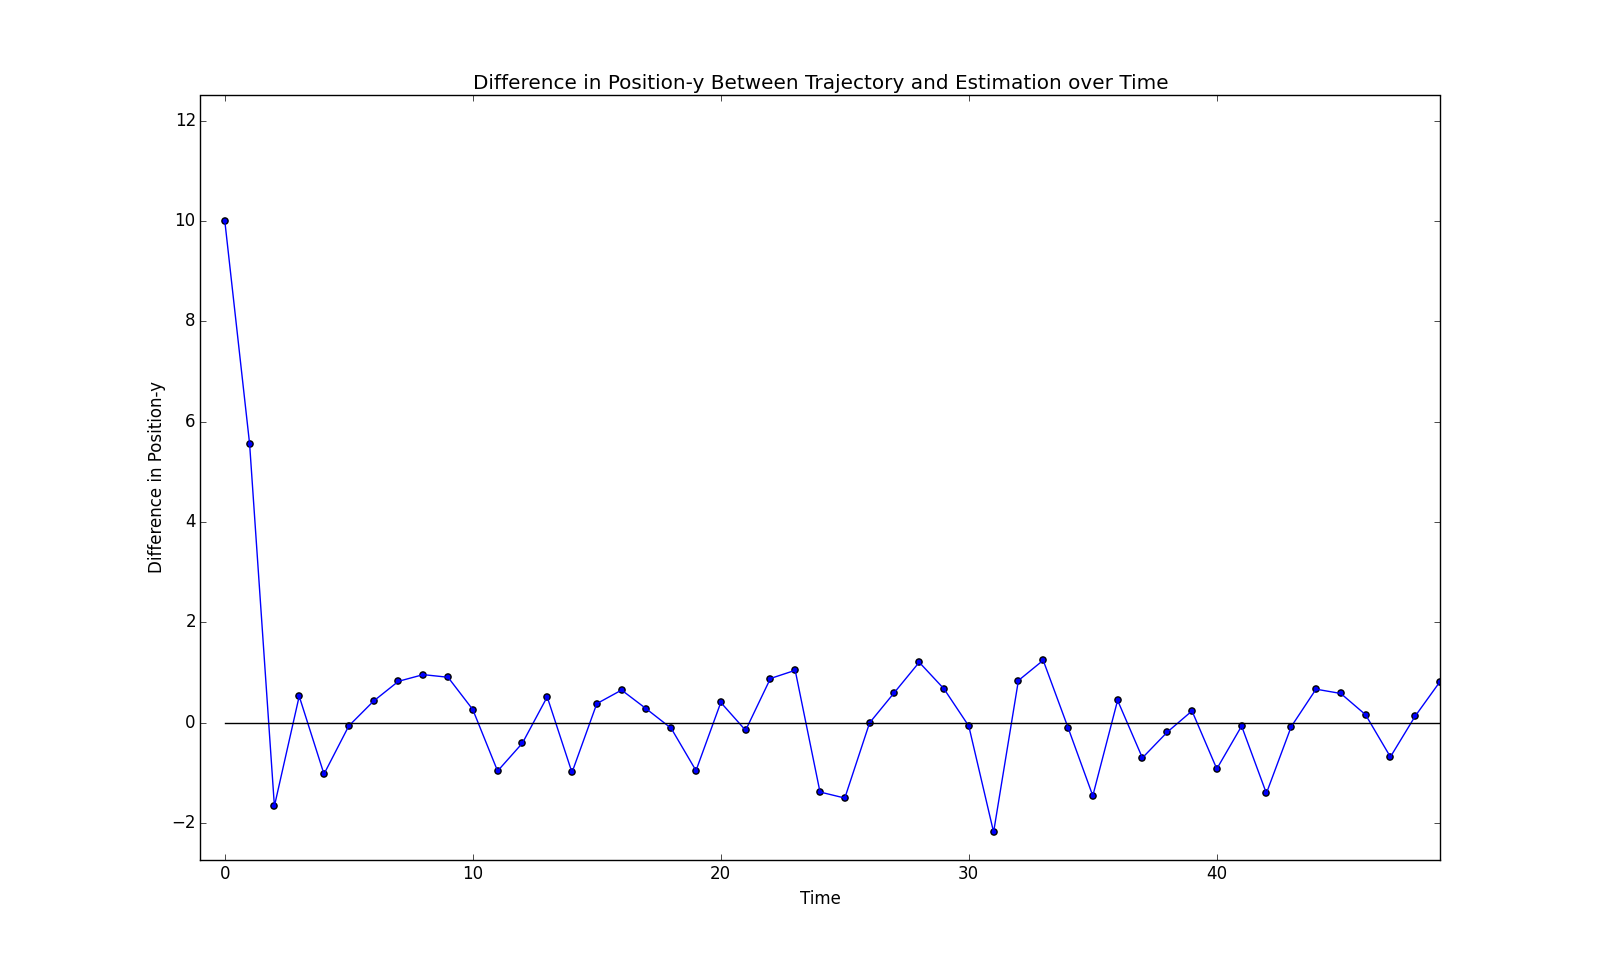
\includegraphics[width=\textwidth]{Diffpy}
		\caption{Difference between real and estimated $y$ position}
	\end{figure}

	\begin{figure}[H]
		\centering
		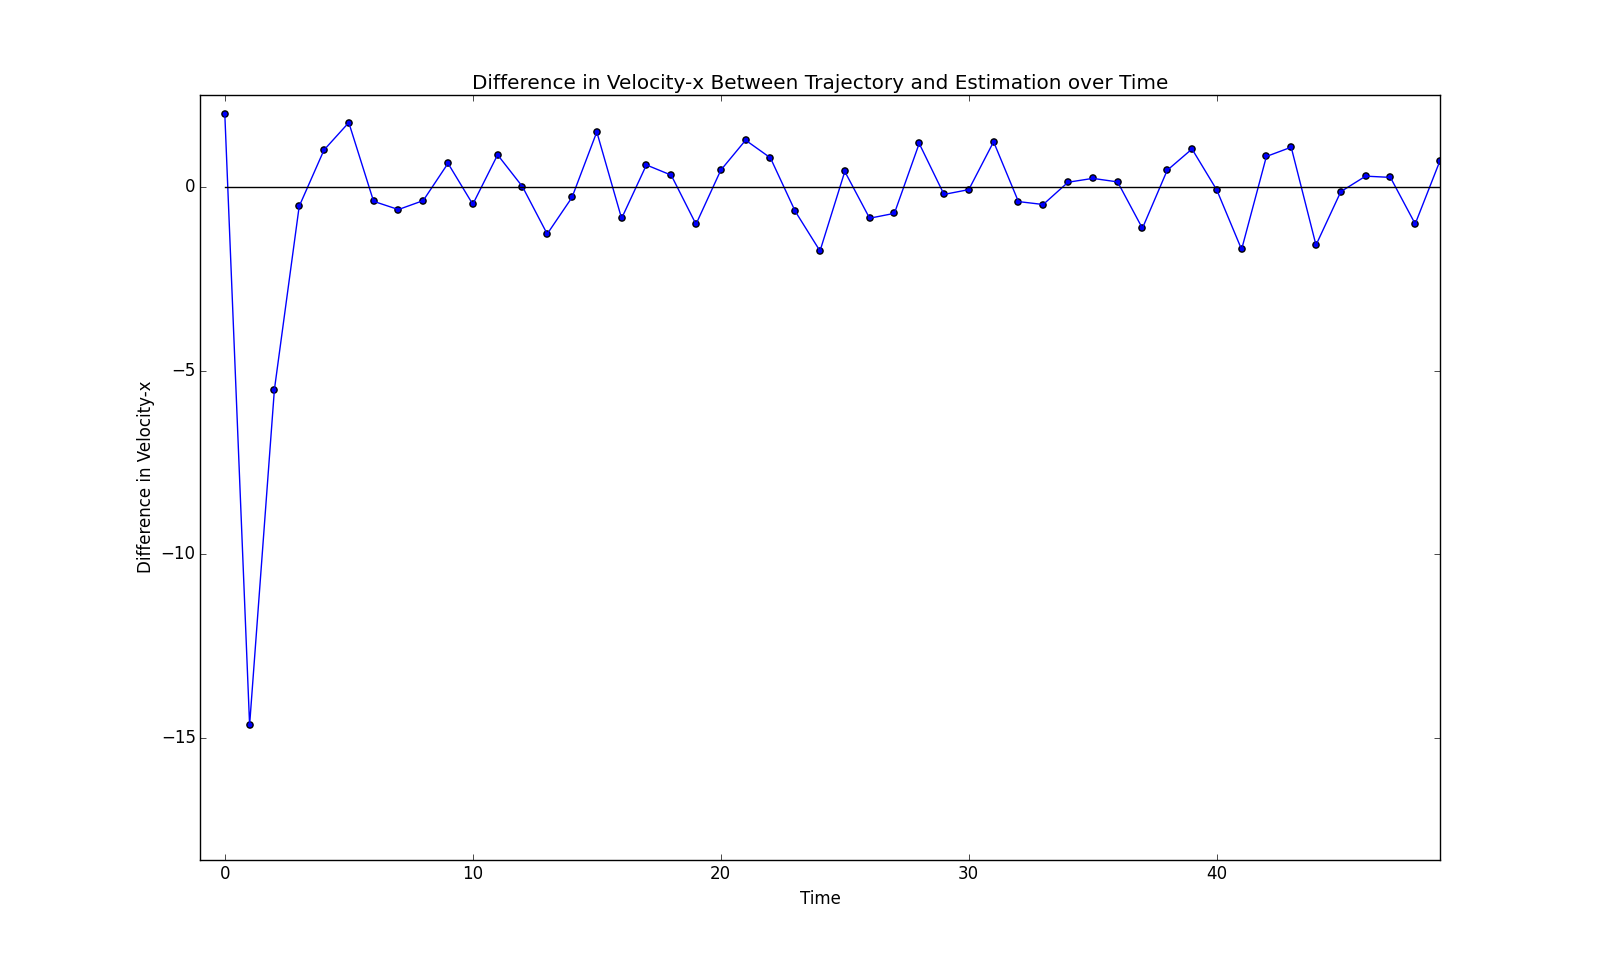
\includegraphics[width=\textwidth]{Diffvx}
		\caption{Difference between real and estimated $x$ velocity}
	\end{figure}

	\begin{figure}[H]
		\centering
		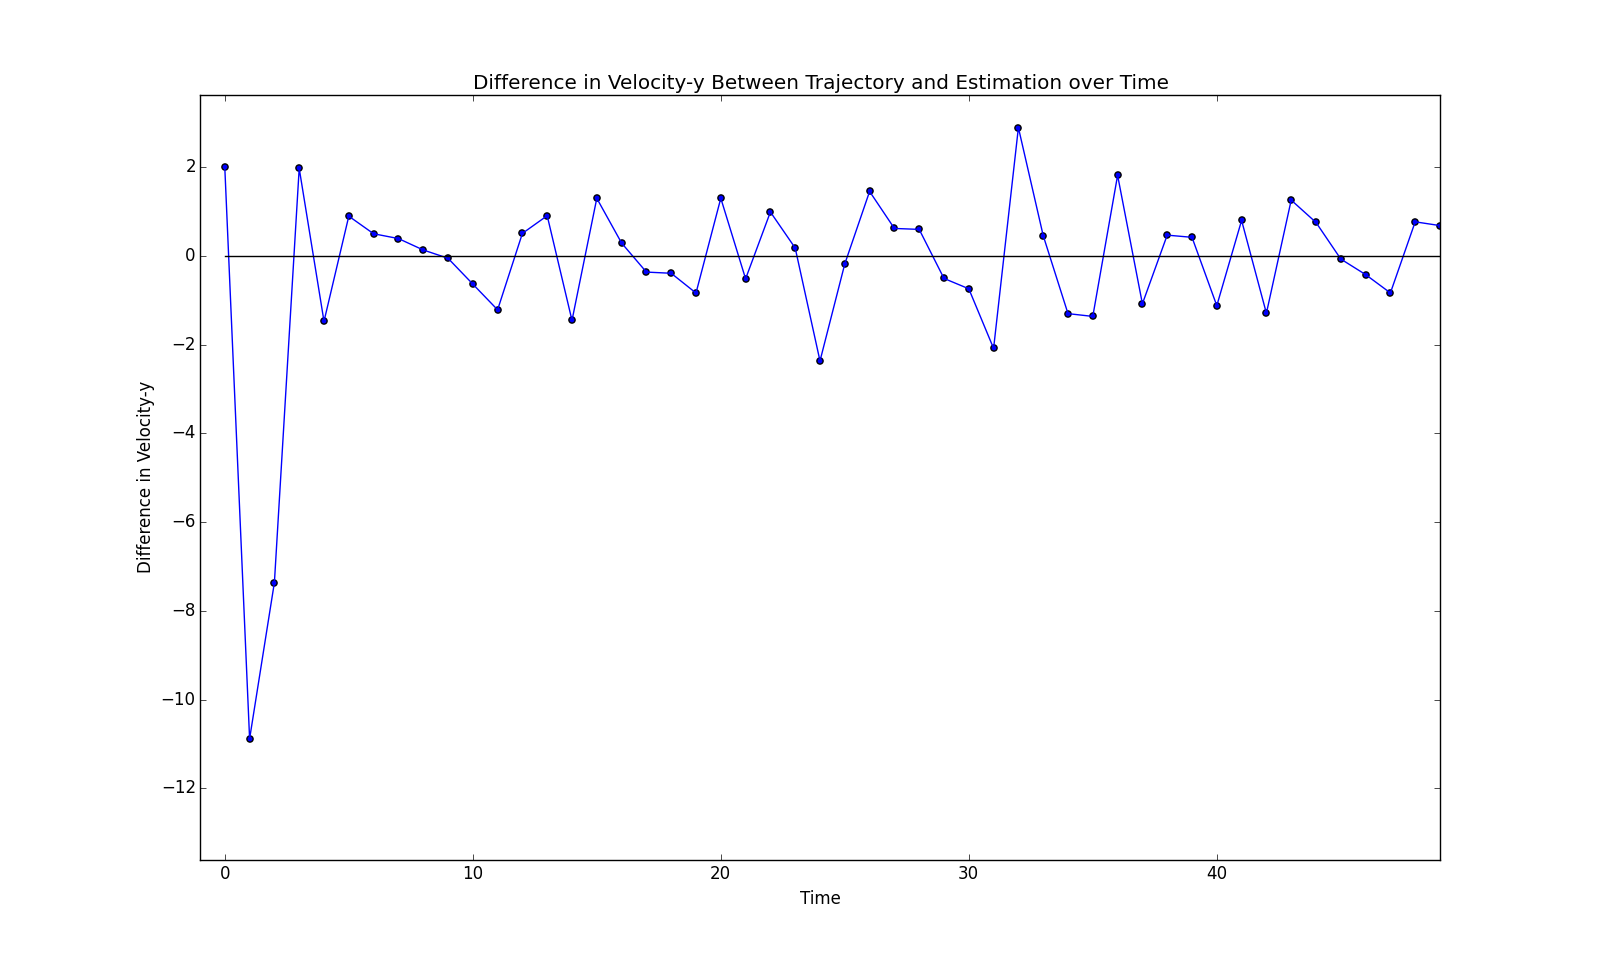
\includegraphics[width=\textwidth]{Diffvy}
		\caption{Difference between real and estimated $y$ velocity}
	\end{figure}
\end{document}
